\documentclass{officialexam} 
\usepackage{chemfig}
\usepackage{tikz}
\usepackage{circuitikz}
\usepackage{graphicx}
\graphicspath{ {./images/} }
\usepackage[version=4]{mhchem}
\definecolor{ffqqqq}{rgb}{1,0,0}
\definecolor{sqsqsq}{rgb}{0.13,0.13,0.13}
\definecolor{ffffff}{rgb}{1,1,1}
\definecolor{uququq}{rgb}{0.25,0.25,0.25}
\everymath{\color{blue}}
\definecolor{qqqqff}{rgb}{0,0,1}
\begin{document}
	\maketitle\\
	\centering{\kml \color{blue}\underline{ប្រធាន:}}
	\begin{enumerate}[I]
		\item (៦ ពិន្ទុ) តើបាតុភូតអូតូអាំងឌុចស្យុងម៉ាញេទិចកើតឡើងនៅពេលណា?
		\item (៦ ពិន្ទុ) ចូររៀបរាបពីវគ្គទាំងបួននៃម៉ាសុីនបន្ទុះបួនវគ្គ។ តើវគ្គណាមួយដែលជាវគ្គបង្កើតកម្មន្តមេកានិច?
		\item (១៥ ពិន្ទុ) នៅភាពដើម $P_i~;~V_i$ និង $T_i$  នៃឧស្ម័នបរិសុទ្ធមួយត្រូវបានឆ្លងកាត់មួយវដ្តនៃដំណើរការដូចបានបង្ហាញក្នុងរូប។
		\begin{multicols}{2}
			\begin{enumerate}[k]
				\item គណនាកម្មន្តសរុបក្នុងមួយវដ្តនៃដំណើរការ។
				\item គណនាបរិមាណកម្តៅសរុបក្នុងមួយវដ្តនៃដំណើរការ។
				\item ចូរអនុវត្តន៍ជាលេខ ដើម្បីគណនាកម្មន្តសរុបក្នុងមួយវដ្តនៃដំណើរការដូចរូប ។ បើ $1.0mol$ នៃឧស្ម័នស្ថិតនៅសីតុណ្ហភាព $0^\circ C$។ \\គេឱ្យ ថេរសកលនៃឧស្ម័ន $R=8.31J/mol\cdot K$
			\end{enumerate}
			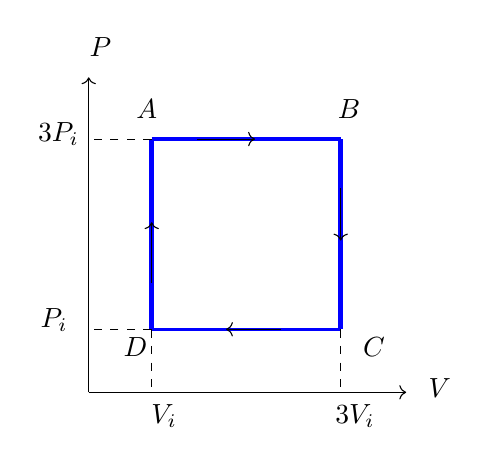
\begin{tikzpicture}[x=1.0cm,y=1.0cm, scale=0.8]
			\draw [->] (-1,0) -- (-1,5);
			\draw [->] (-1,0) -- (4.04,0);
			\draw [line width=1.6pt,color=qqqqff] (0,1)-- (0,4.02);
			\draw [line width=1.6pt,color=qqqqff] (0,4.02)-- (3,4.02);
			\draw [line width=1.6pt,color=qqqqff] (3,4.02)-- (3,1);
			\draw [line width=1.2pt,color=qqqqff] (0,1)-- (3,1);
			\draw [dash pattern=on 3pt off 3pt] (0,1)-- (0,0);
			\draw [dash pattern=on 3pt off 3pt] (3,1)-- (3,0);
			\draw [dash pattern=on 3pt off 3pt] (0,1)-- (-1,1);
			\draw [dash pattern=on 3pt off 3pt] (0,4.02)-- (-1,4.02);
			\draw (-1.14,5.78) node[anchor=north west] {$P$};
			\draw (4.24,0.38) node[anchor=north west] {$V$};
			\draw (-1.96,4.44) node[anchor=north west] {$3P_i$};
			\draw (-1.92,1.48) node[anchor=north west] {$P_i$};
			\draw (-0.16,-0.04) node[anchor=north west] {$V_i$};
			\draw (2.76,-0.04) node[anchor=north west] {$3V_i$};
			\draw [->] (0,1.74) -- (0,2.7);
			\draw [->] (0.72,4.02) -- (1.64,4.02);
			\draw [->] (3,3.24) -- (3,2.41);
			\draw [->] (2.06,1) -- (1.18,1);
			\draw (-0.4,4.80) node[anchor=north west] {$A$};
			\draw (2.80,4.80) node[anchor=north west] {$B$};
			\draw (3.20,1.02) node[anchor=north west] {$C$};
			\draw (-0.6,1.02) node[anchor=north west] {$D$};
			\end{tikzpicture}
		\end{multicols}
		\item (១៥ ពិន្ទុ)  ម៉ូទ័រម៉ាសុីនម៉ាស៊ូតនៃរថយន្តមួយដែលមានទិន្នផលកម្តៅ $0.43$ ហើយវាស្រូបកម្តៅ $4.0MJ$ ពីប្រភពក្តៅ។ គណនា៖
		\begin{enumerate}[k]
			\item កម្មន្តមេកានិចដែលបានពីពីស្តុង។
			\item បរិមាណកម្តៅដែលបញ្ចេញទៅក្នុងបរិយាកាស។
			\item កម្មន្តបានការ បើគេដឹងថាទិន្នផលគ្រឿងបញ្ជូន $0.82$។
		\end{enumerate}
		\item (១៥ ពិន្ទុ) កុងដង់សាទ័រមួយផ្ទុកក្រោមតង់ស្យុង $V=10.0V$ បានផ្ទុកថាមពលស្មើ $4.0mJ$។ កុងដង់សាទ័រនេះបានផ្ទេរបន្ទុកអគ្គិសនីទៅក្នុងបូប៊ីនមួយដែលមានរេសុីស្តង់អាចចោលបាន និងមានអាំងឌុចតង់ $L=2.0mH$។
		\begin{enumerate}[k]
			\item ចូរកំណត់ ខួប ប្រេកង់ និងពុល​​សា​​ស្យុងផ្ទាល់នៃសៀគ្វីយោល $LC$ នេះ។
			\item គណនាអំព្លីទុតនៃចរន្តដែលឆ្លងកាត់បូប៊ីន។
		\end{enumerate}
		\item (១៨ ពិន្ទុ) សូលេណូអុីតមួយមានប្រវែង $l=80.0cm$ អង្កត់ផ្ចិត $D=4.0cm$ ត្រូវបានរុំជា​​ស្ពៀ​​​​ជាប់ៗ​​គ្នាចំនួន $2000$ ស្ពៀ។
		\begin{enumerate}[m]
			\item គណនាអាំងឌុចតង់នៃសូលេណូអុីតនេះ។ គេឱ្យ $~\pi^2=10$ និងជំរាបដែនម៉ាញេទិចក្នុងសុញ្ញាកាស $\mu_0=4\pi\times10^{-7}T\cdot m/A$
			\item គេយកសូលេណូអុីតខាងលើមកតជាស៊េរីជាមួយរេសុីស្តង់មួយដែលមានតម្លៃ $R=4.0\Omega$ រួចភ្ជាប់ទៅនឹងបាតេរី $\varepsilon=V=6.0V$ ដូចបានបង្ហាញក្នុងរូប៖
			\begin{multicols}{2}
				\begin{enumerate}[k]
					\item គណនាថេរពេលនៃសៀគ្វី $RL$
					\item គណនាតម្លៃចរន្តអគ្គិសនីក្នុងរបបអចិ​​ន្រៃ្តយ៍
					\item គណនាចរន្តដែលឆ្លងកាត់សៀគ្វី នៅខណៈ $t=2ms$ និង $t=\infty$ ក្រោយពេលបិទកុងតាក់ $S$។
					គេឱ្យ $e^{-1}=0.367$
				\end{enumerate}
				\includegraphics[scale=0.25]{pic5}
			\end{multicols}
		\end{enumerate} 
	\end{enumerate}
\end{document}